\documentclass{standalone}
\usepackage{tikz}
\usepackage{ctex,siunitx}
\setCJKmainfont{Noto Serif CJK SC}
\usepackage{tkz-euclide}
\usepackage{amsmath}
\usetikzlibrary{patterns, calc,3d}
\usetikzlibrary {decorations.pathmorphing,decorations.pathreplacing,decorations.shapes}
\tikzset{label style/.append style={font=\small}}
\begin{document}
\small
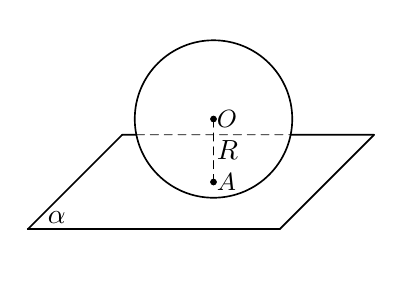
\begin{tikzpicture}[>=latex,scale=0.8,inner sep=1pt]
\useasboundingbox(0,-0.6)rectangle(5.5,3.2); 
  \tkzDefPoints{0/0/Q,4/0/M,5.5/1.5/N,1.5/1.5/P,2.95/0.75/A,2.95/1.75/O}
  \tkzDefShiftPoint[O](0,1.25){R}
  % \tkzInterLC(Q,M)(O,R)\tkzGetPoints{r}{r'}
  \tkzInterLC(N,P)(O,R)\tkzGetPoints{s}{s'}
  \tkzDrawSegments[semithick](P,Q Q,M M,N N,s' s,P)
  \tkzDrawSegments[densely dashed](s,s' O,A)
  \tkzDrawCircle[semithick,black](O,R)
  % \tkzDrawArc[densely dashed](O,R)(r)
  % \tkzDrawArc[semithick](O,r)(r')
  % \tkzDrawArc[densely dashed](O,r')(R')
  % \draw[densely dashed,very thin](R)arc(180:0:1.25 and 0.3);
  % \draw(R)arc(-180:0:1.25 and 0.3);
  \tkzLabelLine[pos=0.5,right](O,A){$R$}
  \tkzDrawPoints[fill=black](O)
  \tkzDrawPoints[fill=black](A)
  \tkzLabelPoints[right](O,A)
  \tkzLabelAngle[pos=0.5](M,Q,P){$\alpha$}
\end{tikzpicture}
\end{document}